%\input{simple_template.tex}
\documentclass{econpaper}


\author[1]{Gabriel Petrini}
\author[2]{Lucas Teixeira}

\affil[1]{PhD student at Unicamp. Email: \url{gpetrinidasilveira@gmail.com}
}
\affil[2]{Assistant-Professor at Unicamp.}


\usepackage{epstopdf}% To incorporate .eps illustrations using PDFLaTeX, etc.
\epstopdfsetup{suffix=}
\usepackage{graphicx}
\usepackage{multirow}
\usepackage{tablefootnote}
\usepackage{threeparttable}
\usepackage{booktabs}
\usepackage{float}
%% The amssymb package provides various useful mathematical symbols

\usepackage[T1]{fontenc}
\usepackage[utf8]{inputenc}%deve ser usado utf8 ao invés de latin1
\usepackage[american]{babel}
\usepackage{setspace}
\usepackage{amssymb}
\usepackage{amsmath}% http://ctan.org/pkg/amsmath
\usepackage{mathptmx}% Times New Roman
\usepackage{url}
\usepackage{caption}
\usepackage{indentfirst}
\usepackage{csquotes}
\usepackage{lipsum}
\usepackage[titletoc,title]{appendix}
%\usepackage{chngcntr} % change counter for appendix

\usepackage{tikz}
\usetikzlibrary{through,calc}


\addbibresource{ref.bib}


\title{Untitled}

\begin{document}
	
\maketitle

\begin{abstract}
	This article investigates the relationship between residential investment, asset inflation, and macroeconomic dynamics based on the US post-deregulation case (1992-2019).
	To do so, we estimate a vector error correction model (VECM) to asses the relevance of real interest rate of real estate. 
	Our results report that housing own interest
	rate explains residential investment growth rate considerably.
	
	\noindent\textbf{Keywords:} Real Estate; own interest rate; Vector Error Correction Model; Sraffian supermultiplier.
\end{abstract}

% Textual

%TODO Add Apostrophe after author citation
%TODO Fix eps generated by subplot
%TODO Fix sum in VEC equation

\input{Introduction.tex}
\section{Housing Dynamics and Business Cycle in the US Economy}\label{sec:Stylized_Facts}

Among aggregate demand expenditures, non-residential investment is one of the most examined (at least) between heterodox macroeconomists.
As a consequence, the relevance of other (autonomous) expenditures on macroeconomic dynamics has been underestimated (\cite{brochier_macroeconomics_2017}).
Residential investment, on the other hand, is not as studied by the literature despite being one of the most volatile expenditure (see Figure \ref{FigVolatilidade}).
Moreover, however small its share on GDP is (see Figure \ref{FigAutonomos}), it does not imply that it has negligible effects on the business cycle.
In this section, we argue that this little attention that residential investment receives is not compatible with its relevance for the US.
Furthermore, we show that this significance is not restricted to the recent housing crisis.

\begin{figure}
	\caption{Housing's Particular Stylized Facts}
	\label{fig:figs}
	\begin{subfigure}[t]{.5\textwidth}
		\centering
		\caption{Selected growth rate distribution (1947-2019)}
		\label{FigVolatilidade}
		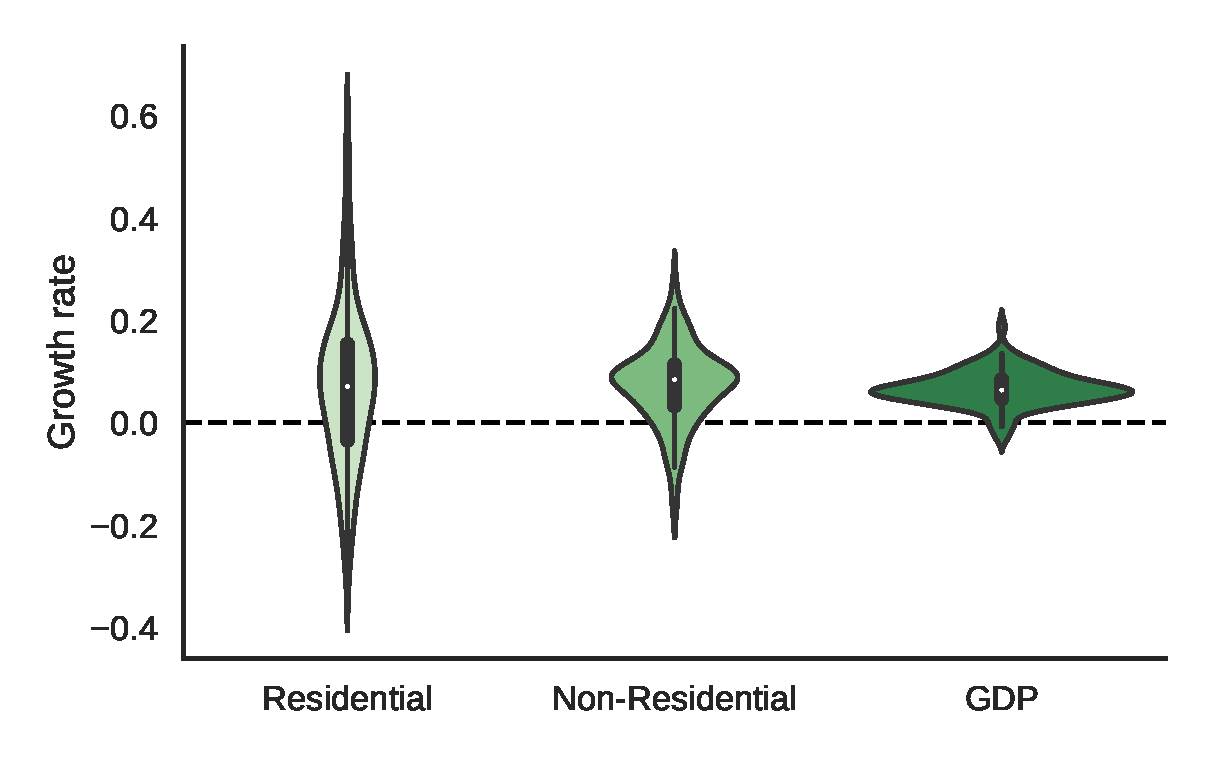
\includegraphics[width=.8\linewidth]{./figs/Volatilidade.eps}
	\end{subfigure}
	\begin{subfigure}[t]{.5\textwidth}
		\centering
		\caption{Autonomous expenditures share on GDP (US, 1979-2019)}
		\label{FigAutonomos}
		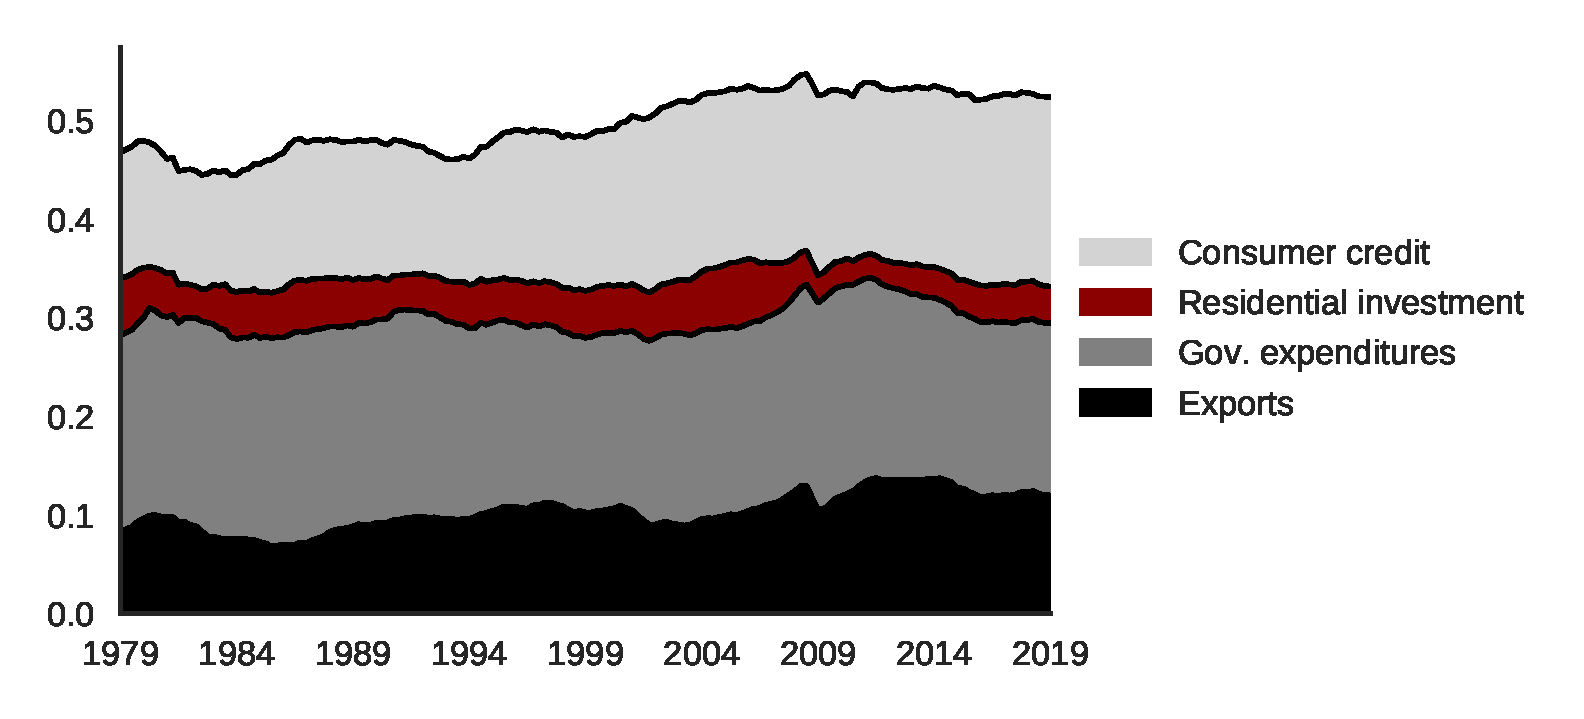
\includegraphics[width=.8\linewidth]{./figs/Gastos_autonomos.eps}  
	\end{subfigure}
	\caption*{\textbf{Source:} U.S. Bureau of Economic Analysis, Authors' Elaboration}
\end{figure}


It is worth mentioning the novelty of \textcite{green_follow_1997} and \textcite{leamer_housing_2007} --- revisited in \textcite{leamer_housing_2015} and by \textcite{fiebiger_trend_2017} --- when shedding light on the relevance of residential investment even before of the Great Recession.
More precisely, \textcite{green_follow_1997} reports that residential investment leads --- more than firms' investment --- the business cycle.
However, argues that this result does not imply a causal relationship:

\begin{quotation}
	[P]erhaps residential investment, like stock prices and interest rates, is a good predictor of GDP because it is a series that reflects \textbf{forward-looking behavior}. Presumably households will not increase their expenditures on housing unless they expect to prosper in the future. Building a house is a natural mechanism for doing this. Thus, the series can do a good job of predicting GDP \textbf{without necessarily causing GDP} (\cite[p.~267, ephasis added]{green_follow_1997}).
\end{quotation}
Despite paying attention to non-capacity creating autonomous expenditure, \textcite{green_follow_1997}, restricts its relevance as temporal precedence indicator.
\textcite{leamer_housing_2007}, on the other hand, reports a causal relationship between housing and GDP.
In summary, states that residential investment implies a higher durable goods consumption, that is, the US business cycle is a ``consumer cycle''.

Next, we present Figure \ref{FigIh_u} in order to depict the relation between housing and business cycle in which each cycle is represented in a different panel\footnote{FIEBIGER}. 
The vertical axis represents residential investment-GDP ratio and the horizontal
axis represents the rate of capacity utilization as a proxy for business cycle.
Economic recovery is generally characterized residential investment growing faster than GDP --- with the 1991-2000 period being a particular case. 
As a consequence of this higher growth rate, is the increase of both residential investment share on GDP and capacity utilization. 
Following the Sraffian supermultiplier growth model, we conclude that increase of non-residential investment is the result of capital stock adjustment principle.
This increase implies GDP to grow faster than residential investment, therefore reducing both its share on GDP and capacity utilization ratio. 
Finally, as a result of economic burst, capacity utilization ratio falls and the cycle.


\begin{figure}[H]
	\centering
	\caption{Residential investment share on GDP VS. capacity utilization during recessions}
	\label{FigIh_u}
	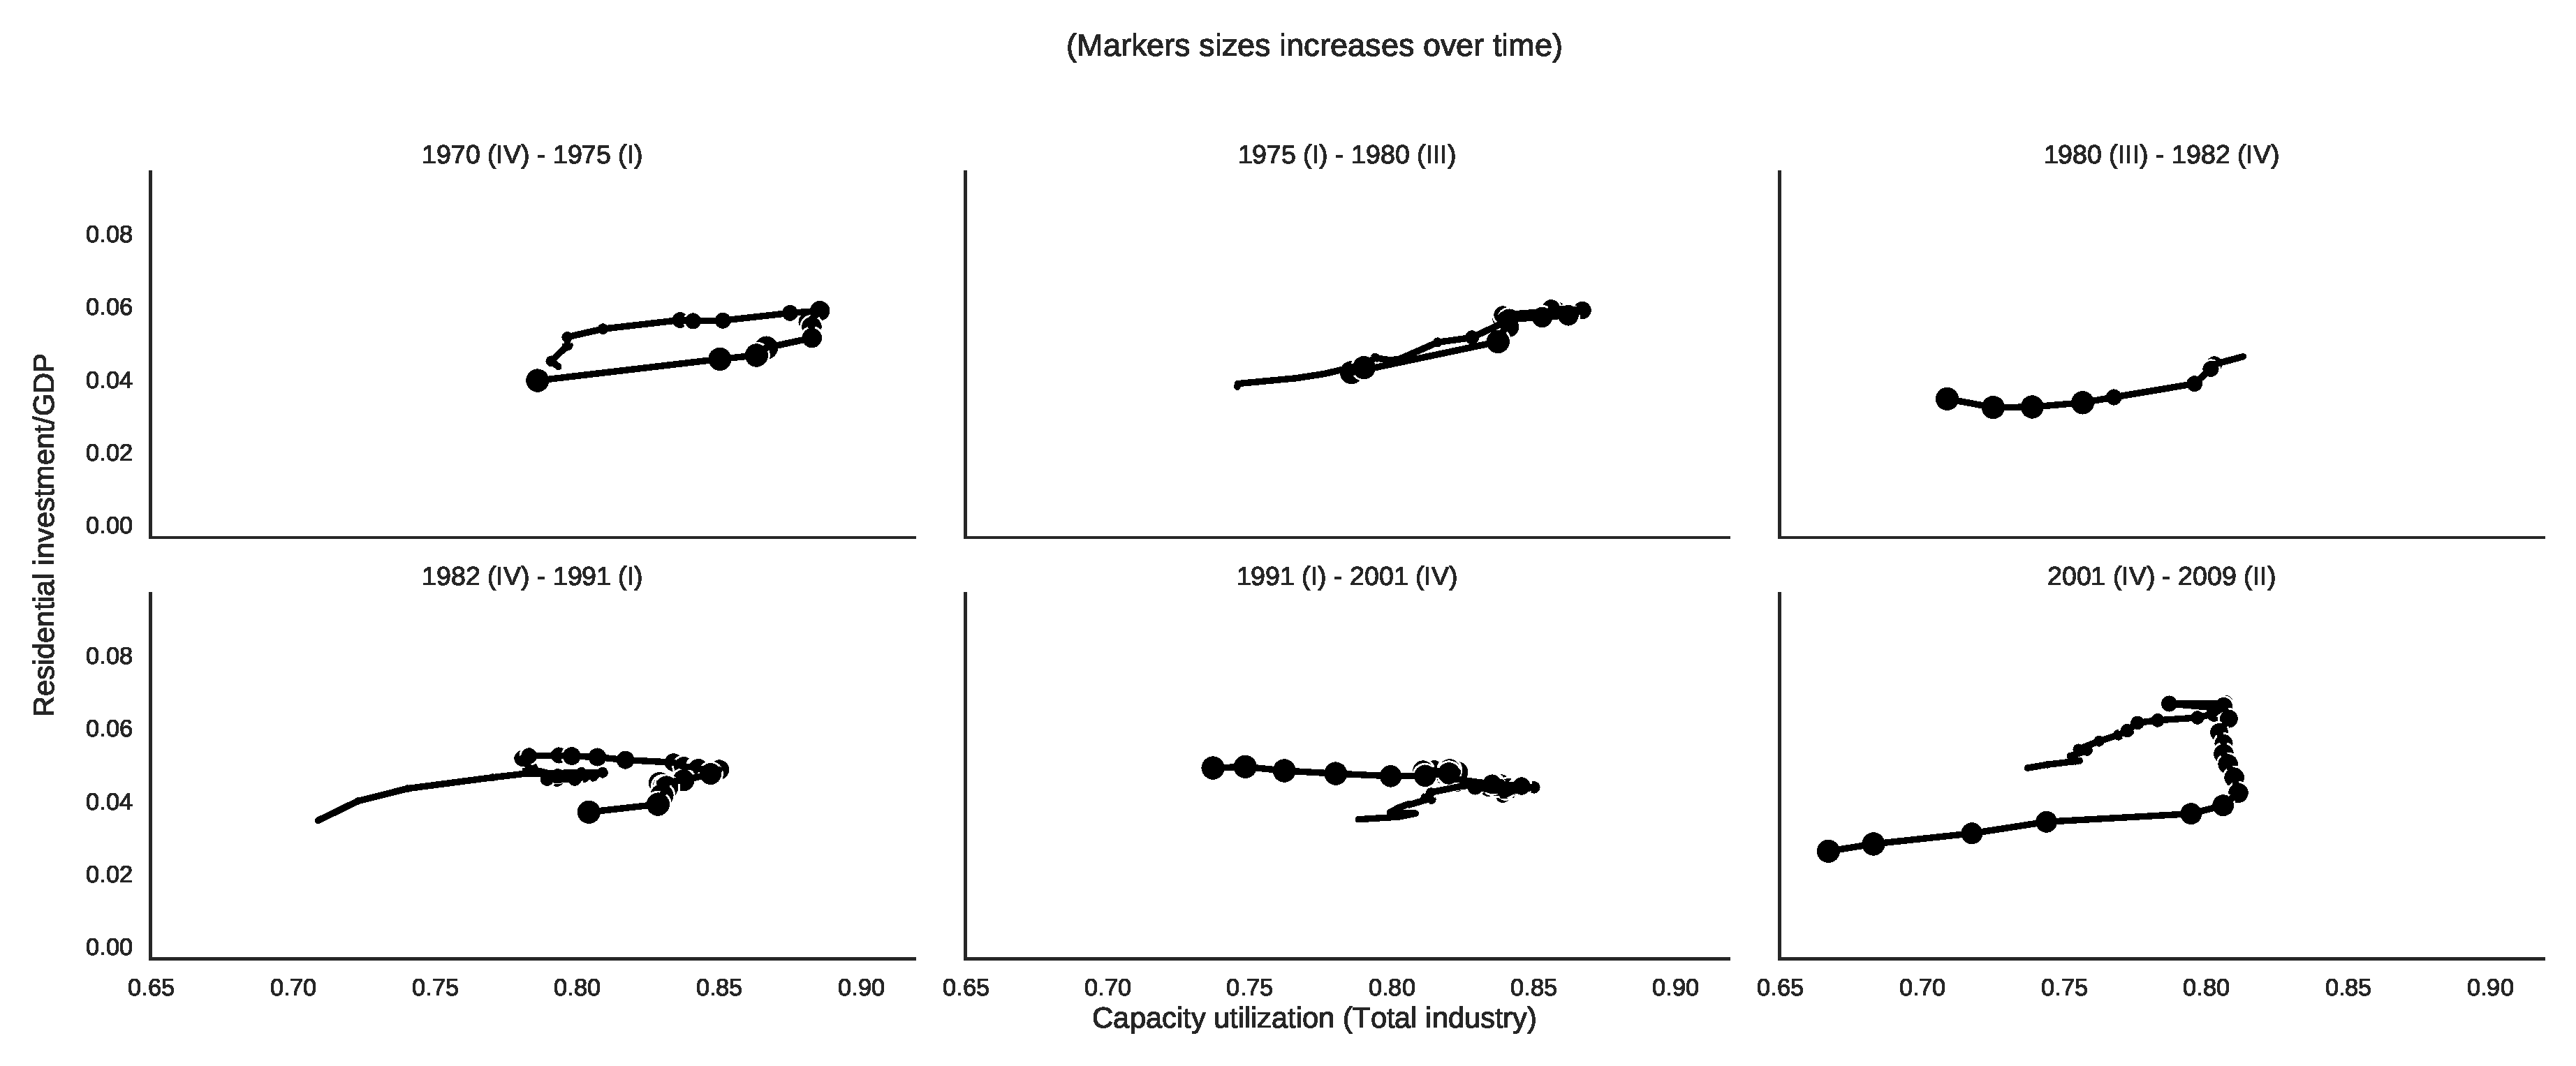
\includegraphics[width=\textwidth]{./figs/Ciclo_Ih_u.eps}
	\caption*{\textbf{Source:} Authors' Elaboration}
\end{figure}

There is also an indirect relation between housing and aggregate demand. 
Real estate constitutes a significant portion of household wealth so houses serves as collateral to borrowing (\cite{teixeira_uma_2011}). 
As a consequence of US institutional arrangement, households --- especially the poorest ones --- could increase their indebtedness as houses prices went up (see Figure \ref{FigDividaPreco}) as a way to ``realize'' capital gains without
selling their homes during house bubble of the 2000s (\cite{teixeira_crescimento_2015}).
Therefore, real estate inflation and durable goods consumption are connected and has relevant consequences for business cycle.
\textcite{zezza_u.s._2008} and \textcite{barba_rising_2009}, for example, report that credit-financed consumption was one of the main drivers of economic growth before the Great Recession.




\begin{figure}[H]
	\centering
	\caption{Household indebtedness and house prices dynamics (jan/2000=100)}
	\label{FigDividaPreco}
	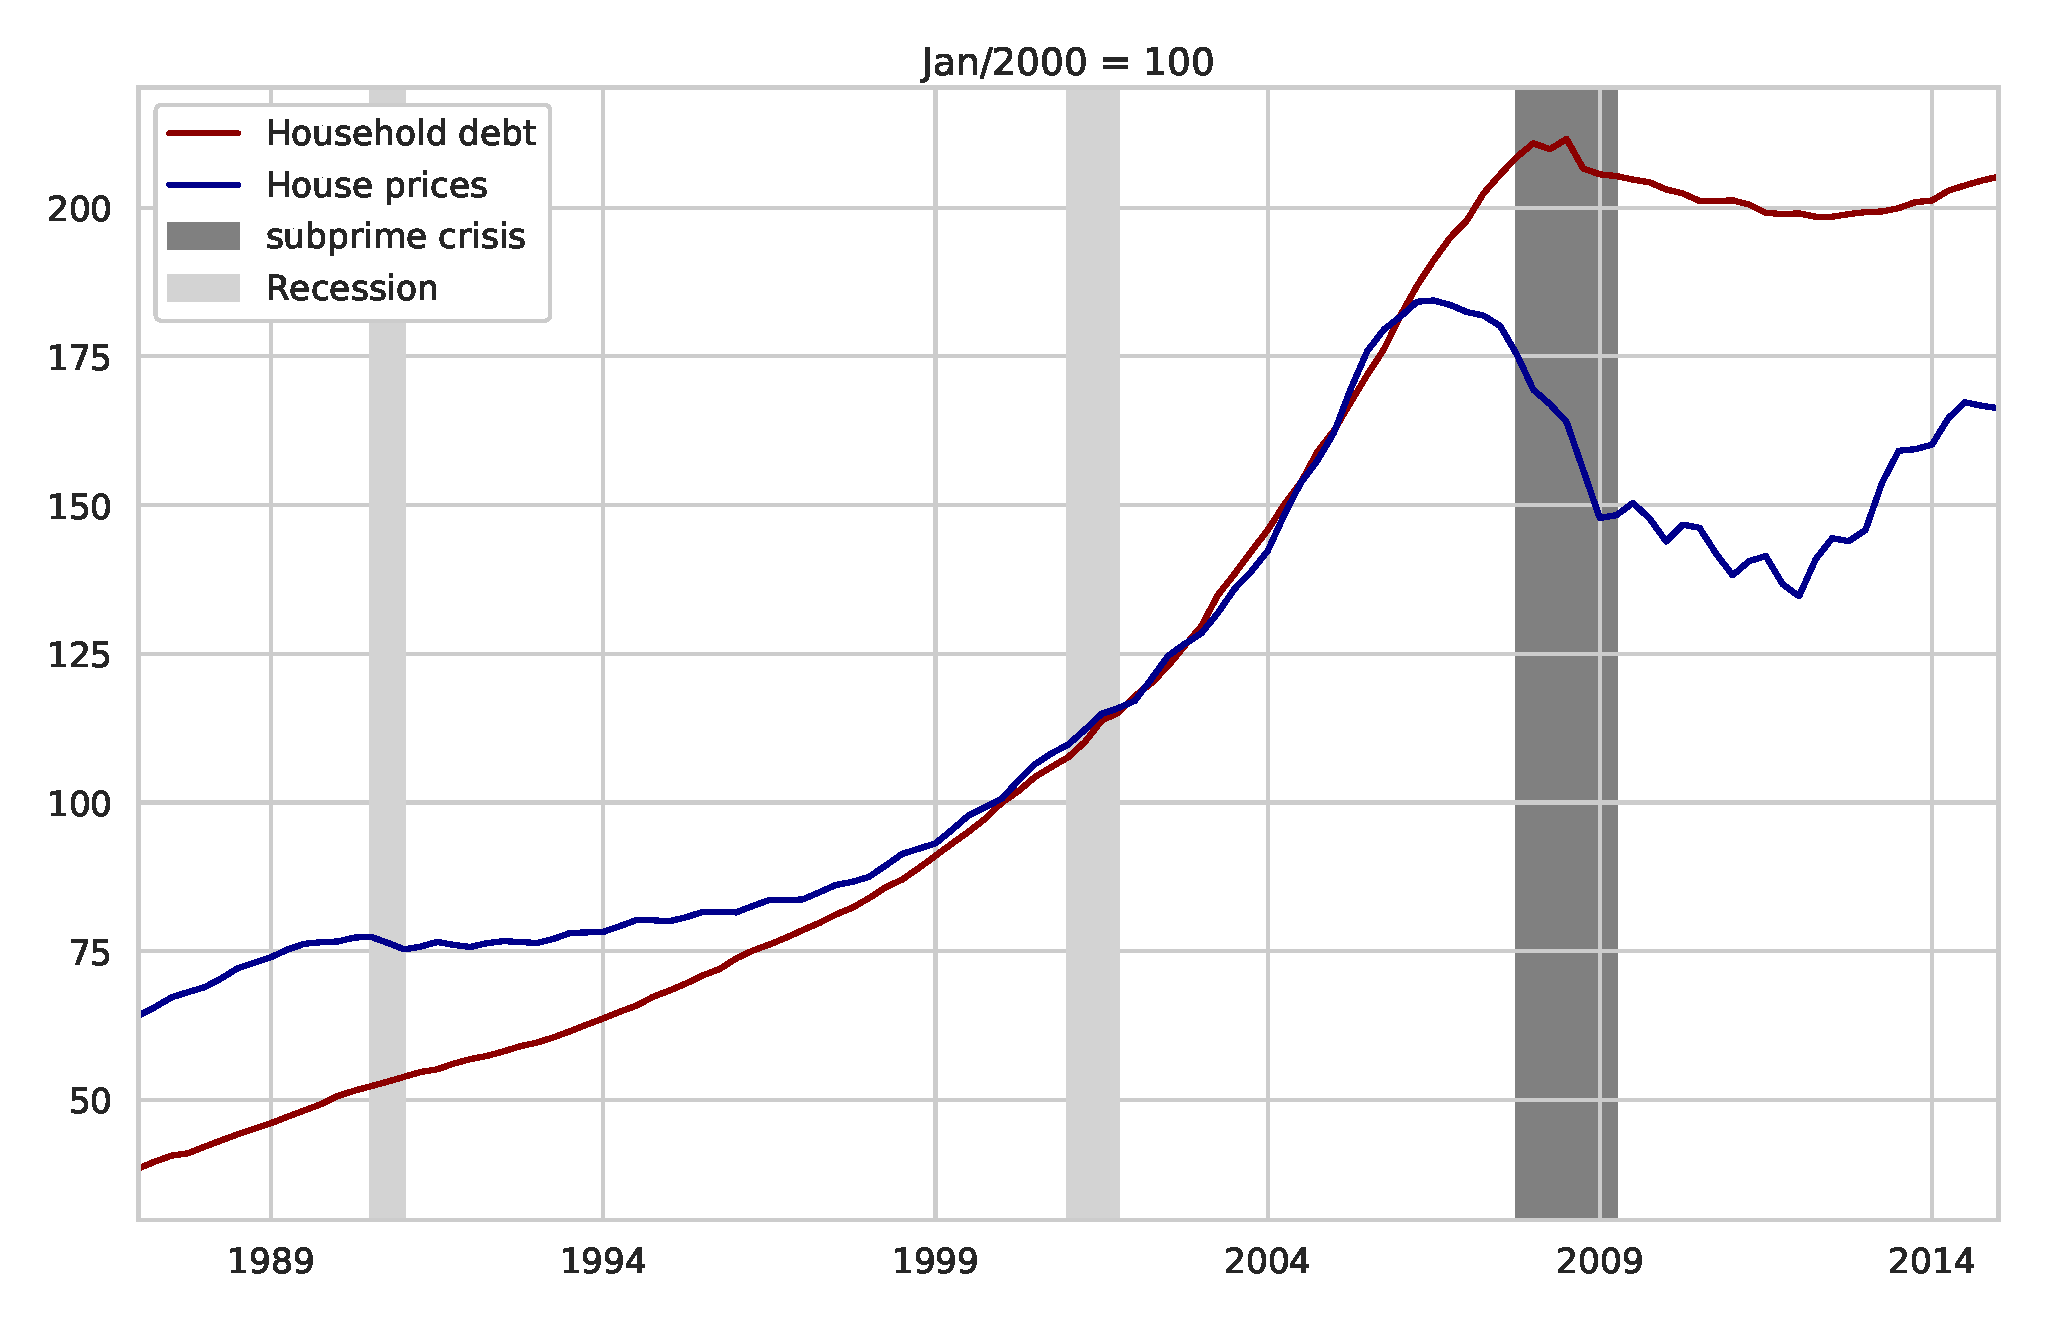
\includegraphics[width=\textwidth]{./figs/Divida_PrecoImoveis.eps}
	\caption*{\textbf{Source:} U.S. Bureau of Economic Analysis, Authors' Elaboration}
\end{figure}
This relation between households indebtedness and real estate inflation has other relevant implications.
The first is the gap between assets and liabilities in the course of the Great Recession.
This dynamic is due both to the housing prices burst (post-2005) and to the insensitivity of households' financial commitments.
In other words, real estate (assets) has a market value while debt (liabilities) has a contractual one, thus, households net worth decreases onset of the subprime crisis.
Therefore, the second implication is the sharp reduction in the net worth of the poorest households in absolute and relative terms (see Figure \ref{FigDistPassivos}).


\begin{figure}
	\centering
	\caption{Liabilities evolution by wealth percentile (1989/07=1)}
	\label{FigDistPassivos}
	\includegraphics[width=.8\textwidth]{./figs/Distribuicao_Passivos.eps}
	\caption*{\textbf{Source:} \textcite{us_census_bureau_characteristics_2017}, Authors' Elaboration}
\end{figure}

In summary, we conclude that housing is relevant to understand the specificity of US business cycle.
On the following section, we analyze how econometric literature has dealt with the topic.
More precisely, we evaluate macroeconometric works according to its compatibility with Sraffian supermultiplier growth model.

\input{Empirical_Review.tex}
\section{Modelo}
\label{Modelo_empirico}

O modelo a ser estimado pretende testar se a taxa própria de juros dos imóveis contribui para explicar a dinâmica do investimento residencial tal como proposto por \textcite{teixeira_crescimento_2015}\footnote{Vale pontuar que tal como no modelo do supermultiplicador sraffiano, a distribuição de renda é determinada por fatores socio-históricos e institucionais e, portanto, não será estimada de modo a manter a consistência teórica.}. Por se tratar de taxas de crescimento com ampla volatilidade, aplicou-se a transformação de \textcite{yeo_new_2000} para conter a amplitude das séries decorrente da crise imobiliária. A razão de se utilizar tal procedimento e não a transformação de \textcite{box_analysis_1964} é por não se restringir a valores não-negativos. Em seguida, foram realizados testes de cointegração de \textcite{engle_co-integration_1987} bem como o procedimento de \textcite{johansen_estimation_1991} e, a um nível de significância de 5\%, conclui-se que as séries são cointegradas e, portanto, é possível estimar um modelo vetor de correção de erros (VECM)\footnote{Os resultados de todos os testes realizados bem como as rotinas utilizadas estão disponíveis sob solicitação.}.

Dito isso, resta determinar a defasagem utilizada. Pelos critérios de informação, tanto para o segundo (trimestre) quanto para o quinto \textit{lag} são elegíveis. Apesar de parcimonioso, a escolha da segunda defasagem não é possui respaldo teórico e isso pode ser visualizado pelo gráfico \ref{meses}. Se considerar o tempo médio de construção de imóveis desde a aprovação até a conclusão, verifica-se que deve-se incluir \textit{ao menos} o segundo \textit{lag} para incorporar as residências construídas para a venda uma vez que tal motivação só é realizada se concluída a construção. 


\begin{figure}[htb]
	\centering
	\caption{Tempo médio de construção (aprovação a conclusão) de imóveis para uma unidade familiar por propósito de construção exceto casas pré-fabricadas (1976-2018)}
	\label{meses}
	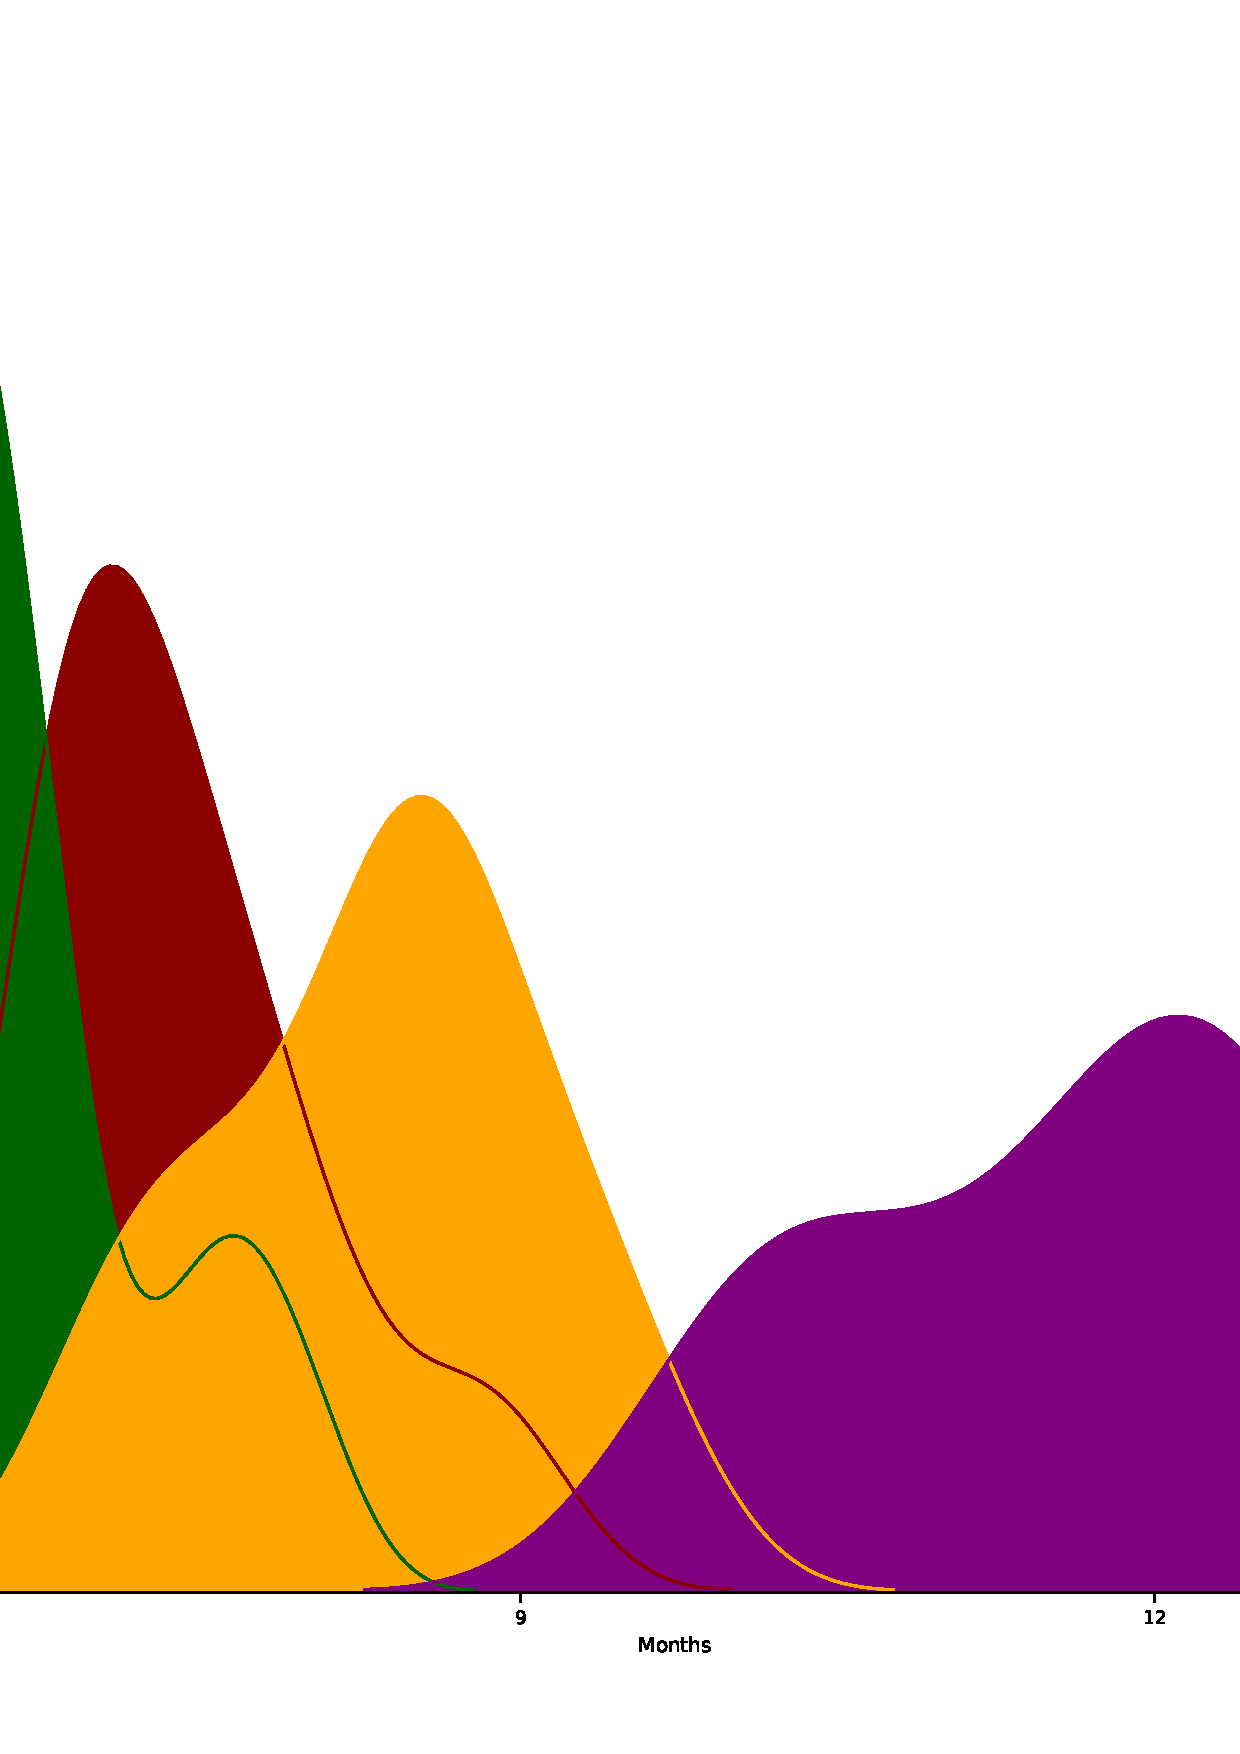
\includegraphics[width=\textwidth]{Fatos_Estilizados/Figs/Meses_contrucao.png}
	\caption*{\textbf{Fonte:} Survey of Construction (SOC), elaboração própria}
\end{figure}
Tal procedimento, no entanto, não é suficiente para determinar a seleção do \textit{lag} a ser utilizado. Dado que o fluxo de novos imóveis é significativamente inferior ao estoque existente, o efeito da variação dos preços se verifica mesmo com as construções não concluídas, ou seja, impacto decorre das residências concluídas anteriormente. Desse modo, a justificativa mais razoável é por meio do comportamento \textit{forward looking} reportado por \textcite{green_follow_1997}, ou seja, o processo decisório para iniciar a construção de um novo imóvel depende de componentes expectacionais. Tal elemento é captado pela taxa própria \textit{esperada}. 

De forma a ilustrar tal relação, o gráfico \ref{defasagens} apresenta as variáveis de interesse frente ao \textit{lag} que minimiza os critério AIC e FPE. Esse procedimento permite visualizar se existe alguma relação entre a taxa própria esperada (taxa efetiva defasada) e taxa de crescimento dos imóveis\footnote{De modo a dar conta de não-linearidades, é apresentada a regressão quadrática entre ambas as variáveis (e o mesmo foi realizado para o gráfico inverso).}. Já a relação inversa, qual seja, da taxa de crescimento para a taxa própria não se verifica uma vez que, como visto, o fluxo de novos imóveis é bastante inferior o estoque de imóveis existente e, portanto, é esperado que tal relação não esteja presente. Em outras palavras, a especulação com o \textit{estoque}  de imóveis gera inflação desses ativos que, por conseguinte, afeta a construção de novos imóveis (\textit{fluxo}) e não o inverso. Essa inspeção, portanto, ilustra de forma bastante grosseira tal componente expectacional.  Dito isso,  estima-se um VECM de ordem 5 cujos resíduos são apresentados no gráfico \ref{residuos}\footnote{Nota-se que tal defasagem, além de ser teoricamente justificada também gera resíduos não heterocedásticos, normalmente distribuídos e sem correlação serial.}.

\begin{figure}[htb]
	\centering
	\caption{Dispersão entre taxa própria e crescimento do investimento residencial: defasagens selecionadas a partir dos critérios de informação}
	\label{defasagens}
	\includegraphics[width=\textwidth]{Fatos_Estilizados/Figs/Scatter_VECM.png}
	\caption*{\textbf{Fonte:} Elaboração própria}
\end{figure}
%TODO Adicionar gráficos com defasagem 2


\begin{figure}[htb]
	\centering
	\caption{Inspeção dos resíduos da estimação}
	\label{residuos}
	\includegraphics[height=.4\textheight]{Fatos_Estilizados/Figs/Residuos_4VECM.png}
	\caption*{\textbf{Fonte:} Elaboração própria}
\end{figure}



\begin{center}
	\begin{table}[htb]
		\centering
		\caption{Parâmetros para a equação da Taxa Própria}
	\begin{tabular}{lccclcc}
		\toprule
		\textbf{Equação:} Taxa Prórpia & \textbf{coef} & \textbf{std err} & \textbf{z} & \textbf{P$> |$z$|$} & \textbf{[0.025} & \textbf{0.975]}  \\
		\midrule
		\textbf{$L^1 $ Taxa Própria} &       0.9320  &        0.089     &    10.511  &         0.000***        &        0.758    &        1.106     \\
		\textbf{$L^1 $ gZ}           &      -0.0545  &        0.014     &    -3.786  &         0.000***        &       -0.083    &       -0.026     \\
		\textbf{$L^2 $ Taxa Própria} &      -0.2810  &        0.122     &    -2.305  &         0.021**        &       -0.520    &       -0.042     \\
		\textbf{$L^2 $ gZ}           &       0.0040  &        0.013     &     0.309  &         0.758        &       -0.021    &        0.029     \\
		\textbf{$L^3 $ Taxa Própria} &       0.0043  &        0.127     &     0.034  &         0.973        &       -0.245    &        0.253     \\
		\textbf{$L^3 $ gZ}           &      -0.0132  &        0.012     &    -1.058  &         0.290        &       -0.038    &        0.011     \\
		\textbf{$L^4 $ Taxa Própria} &      -0.0626  &        0.126     &    -0.497  &         0.619        &       -0.309    &        0.184     \\
		\textbf{$L^4 $ gZ}           &      -0.0030  &        0.012     &    -0.242  &         0.809        &       -0.027    &        0.021     \\
		\textbf{$L^5 $ Taxa Própria} &       0.0144  &        0.093     &     0.156  &         0.876        &       -0.167    &        0.196     \\
		\textbf{EC1} &      -0.0099  &        0.007     &    -1.339  &         0.181        &       -0.024    &        0.005     \\
		\textbf{$\beta_1$ } &       1.0000  &            0     &         0  &         0.000***        &        1.000    &        1.000     \\\bottomrule
	\end{tabular}
\caption*{\textbf{Fonte:} Elaboração própria}
\end{table}
\end{center}
	
	\begin{table}[htb]
		\begin{center}
		\caption{Parâmetros para a equação da $g_Z$}	
	\begin{tabular}{lccclcc}
		\toprule
		\textbf{Equação:} $g_Z$ & \textbf{coef} & \textbf{std err} & \textbf{z} & \textbf{P$> |$z$|$} & \textbf{[0.025} & \textbf{0.975]}  \\
		\midrule
		\textbf{$L^1 $ Taxa Própria} &      -0.8392  &        0.553     &    -1.517  &         0.129        &       -1.924    &        0.245     \\
		\textbf{$L^1 $ gZ}           &       0.1290  &        0.090     &     1.435  &         0.151        &       -0.047    &        0.305     \\
		\textbf{$L^2 $ Taxa Própria} &      -1.6629  &        0.761     &    -2.186  &         0.029**        &       -3.154    &       -0.172     \\
		\textbf{$L^2 $ gZ}           &      -0.0663  &        0.081     &    -0.817  &         0.414        &       -0.225    &        0.093     \\
		\textbf{$L^3 $ Taxa Própria} &       1.5635  &        0.793     &     1.972  &         0.049**        &        0.009    &        3.118     \\
		\textbf{$L^3 $ gZ}           &       0.1092  &        0.078     &     1.407  &         0.159        &       -0.043    &        0.261     \\
		\textbf{$L^4 $ Taxa Própria} &      -0.5929  &        0.785     &    -0.755  &         0.450        &       -2.132    &        0.946     \\
		\textbf{$L^4 $ gZ}           &      -0.4590  &        0.078     &    -5.895  &         0.000***        &       -0.612    &       -0.306     \\
		\textbf{$L^5 $ Taxa Própria} &      -0.3158  &        0.577     &    -0.547  &         0.584        &       -1.447    &        0.816     \\
		\textbf{$L^5 $ gZ}           &       0.0265  &        0.089     &     0.299  &         0.765        &       -0.147    &        0.200     \\
		\textbf{EC1} &       0.1388  &        0.046     &     3.021  &         0.003**        &        0.049    &        0.229     \\
		\textbf{$\beta_2$ } &      -0.4833  &        0.230     &    -2.099  &         0.036**        &       -0.934    &       -0.032     \\\bottomrule
	\end{tabular}
\caption*{\textbf{Fonte:} Elaboração própria}
\end{center}
\end{table}
Adotando um nível de significância de 5\%, verifica-se que o parâmetro de correção de erro (referente ao curto prazo) é estatisticamente significante para a equação da taxa de crescimento do investimento residencial enquanto o vetor de cointegração (referente ao longo prazo) é estatisticamente significante para ambas as equações. Seguindo a proposição de \textcite{teixeira_crescimento_2015}, espera-se que os coeficientes da equação $g_Z$ para a taxa própria sejam negativos e este não é o caso apenas para uma das defasagens. Além disso, espera-se que não exista uma relação de curto prazo entre a taxa própria e $g_Z$, ou seja, taxa própria seja fracamente exógena e isso também é verificado. Portanto, os resultados obtidos estão em linha com os esperados. 

Outra forma de verificar a capacidade explicativa da taxa própria para $g_Z$ é por meio da decomposição da variância da previsão (FEVD) como no gráfico \ref{fevd}. Verifica-se que desde o primeiro trimestre a taxa própria contribui para $g_Z$ enquanto o inverso não é válido. Adicionalmente, é notável que tal contribuição é crescente e maior que 50\% para além do 8º trimestre. Portanto, a taxa própria é explicada principalmente por ela mesma e explica $g_Z$ consideravelmente.

\begin{figure}[htb]
	\centering
	\caption{Decomposição da variância da previsão}
	\label{fevd}
	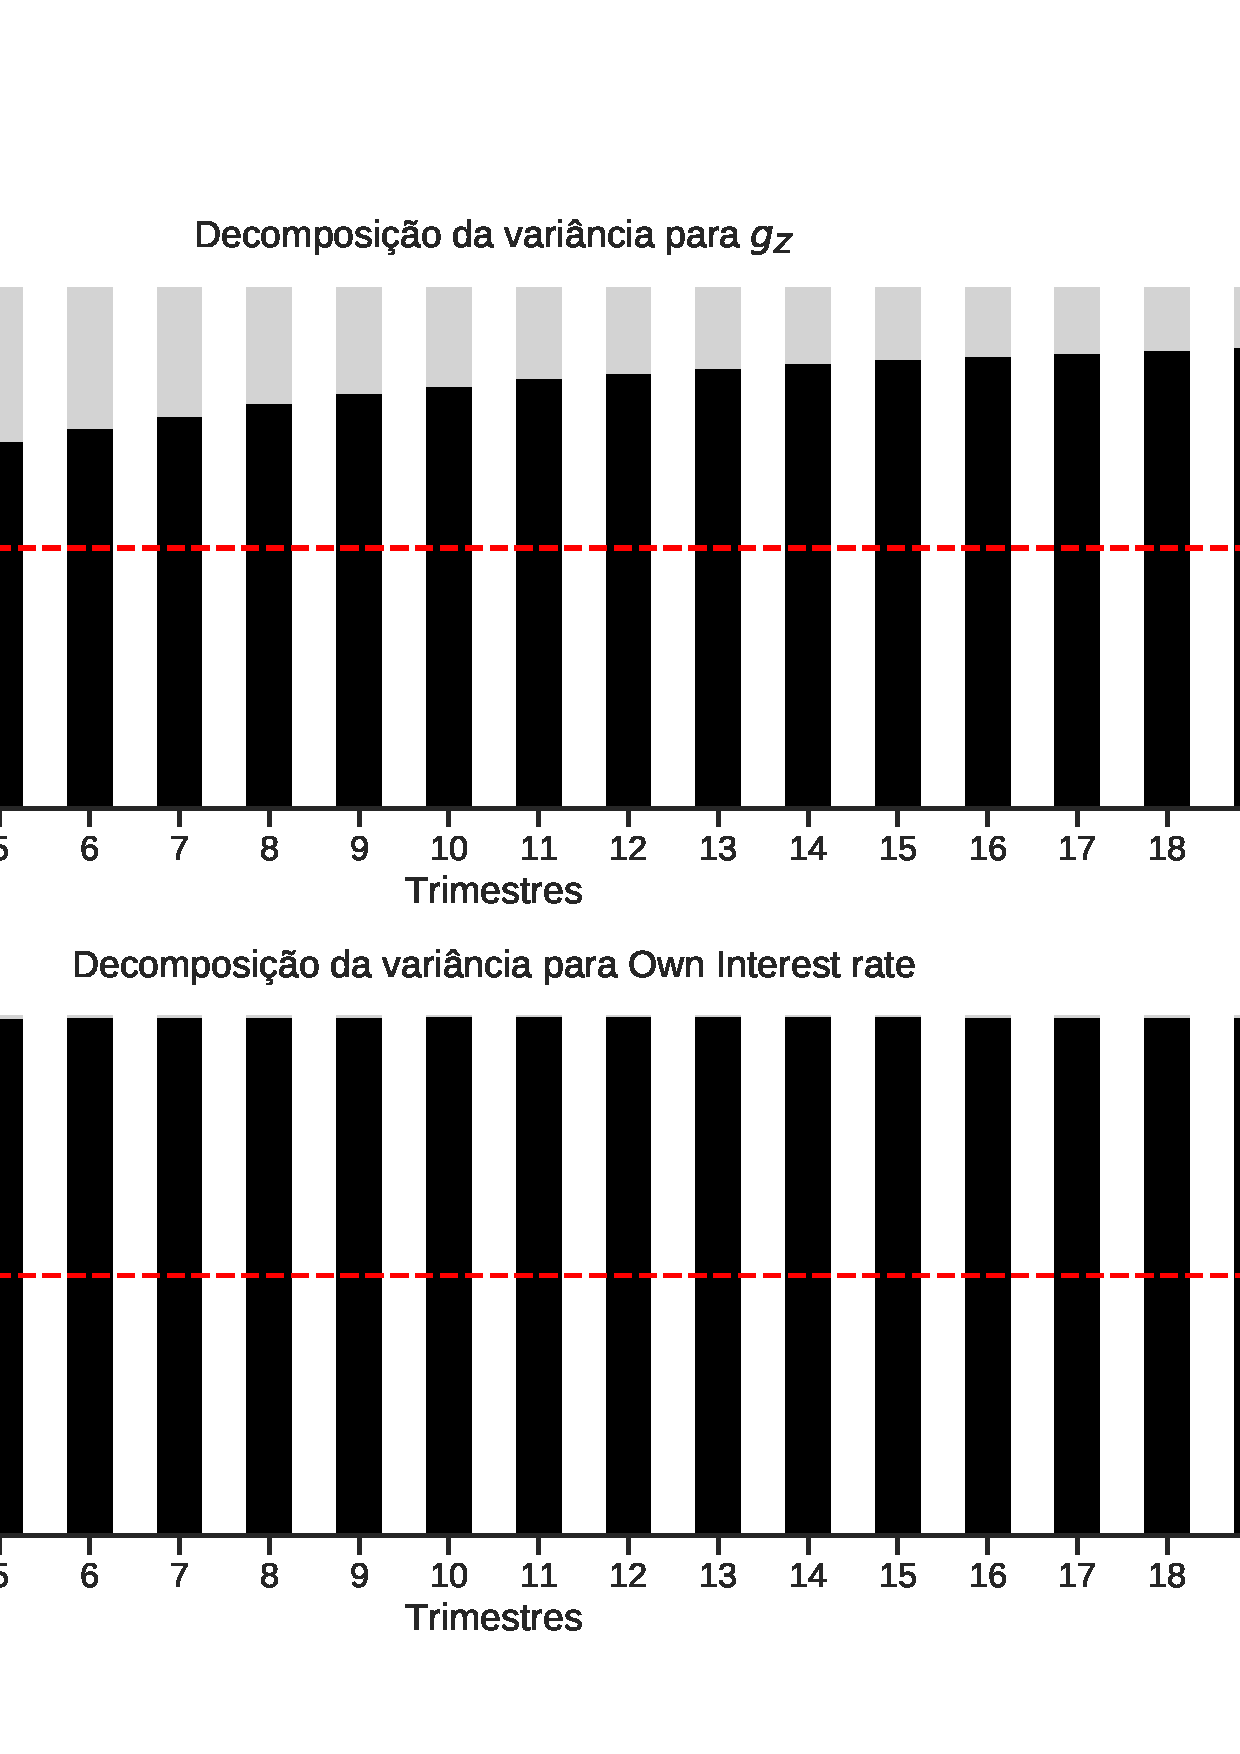
\includegraphics[width=\textwidth]{Fatos_Estilizados/Figs/FEVD_VECM.png}
	\caption*{\textbf{Fonte:} Elaboração própria}
\end{figure}

Adiante, é apresentado o gráfico da função impulso resposta ortogonalizada. Grosso modo, as conclusões da FEVD se estendem para os choques. Os efeitos do aumento da taxa própria é positivo sobre ela mesma e se amortece ao longo do tempo, evidenciando um sistema estável e o mesmo vale para os efeitos do aumento de $g_Z$ sobre $g_Z$. Já os efeitos de $g_Z$ sobre a taxa própria é negativo no curto prazo mas se dissipa para além do 5º trimestre uma vez que passa a pertencer ao intervalo de confiança. A explicação desse resultado decorre dos efeitos de $g_Z$ sobre o preço dos imóveis (diminuição da Taxa Própria) uma vez que a taxa de juros das hipotecas é mantida constante. Por fim, e este é o resultado relevante, dados os objetivos, é o efeito negativo considerável e duradouro (6 trimestres) da taxa própria sobre $g_Z$, confirmando a tese de \textcite{teixeira_crescimento_2015}, e que se torna positivo em um horizonte mais longo podendo estar associado a construção de novos imóveis por motivos não-especulativos decorrentes da redução da inflação imobiliária (aumento da taxa própria).
%alinhado com os resultados de \textcite{huang_is_2018} para o longo prazo.
%podendo estar associado aos gastos com aprimoramento residencial uma vez encerradas as construções (também contabilizado como investimento residencial).

%TODO Rever efeito positivo no longo prazo

\begin{figure}[htb]
	\centering
	\caption{Função impulso resposta ortogonalizada}
	\label{fevd}
	\includegraphics[width=\textwidth]{Fatos_Estilizados/Figs/Impulso_VECM.png}
	\caption*{\textbf{Fonte:} Elaboração própria}
\end{figure}

Dos resultados apresentados acima, verifica-se que a taxa própria de juros dos imóveis tem uma capacidade explicativa significativa. Vale destacar que apesar de amplitude das defasagens selecionadas, o modelo estimado é bastante parcimonioso em termos das variáveis utilizadas. Desse modo, considerando o grau de parcimônia e a robustez dos resultados, conclui-se que é um modelo satisfatório para explicar a taxa de crescimento dos imóveis. Diante da qualidade do ajuste, o gráfico \ref{previsao} apresenta a previsão do modelo 4 passos a frente. Avaliando o últimos resultados disponíveis das contas nacionais e estimativas da taxa própria, verifica-se uma previsão satisfatória uma vez que tanto $g_Z$ reduz quanto a taxa própria aumenta.

\begin{figure}[htb]
	\centering
	\caption{Previsão 4 passos a frente}
	\label{previsao}
	\includegraphics[width=\textwidth]{Fatos_Estilizados/Figs/Previsao_VECM.png}
	\caption*{\textbf{Fonte:} Elaboração própria}
\end{figure}

\section{Concluding Remarks}\label{sec:Conclusion}

\section*{Acknowledgments}

\noindent We are grateful to  Rosângela Ballini, Carolina Baltar, Júlia Braga, Ítalo Pedrosa, Cecon/Unicamp and UFRJ Macroeconomic discussion groups for useful comments and suggestions on earlier drafts of this article. All remaining errors are, of course, our own.

\section*{Disclosure statement}

\noindent No potential conflict of interest was reported by the authors.


\printbibliography{}

\begin{appendix}
	\section{Numerical Appendix}\label{Appen:A}
\end{appendix}

\end{document}